% !TEX TS-program = xelatex
% !TEX encoding = UTF-8 Unicode
% !Mode:: "TeX:UTF-8"
%
% English counterpart of resume-zh_CN.tex. Keep the two in sync when editing.

\documentclass{resume}
\usepackage{zh_CN-Adobefonts_external} % so stray CJK (names, labs) still renders
\usepackage{linespacing_fix} % disable extra space before next section
\usepackage{cite}
\usepackage{tabu}
\usepackage{multirow}
\usepackage{adjustbox}
\hypersetup{
hidelinks,
colorlinks=true,
linkcolor=purple,
citecolor=purple
}

% Tighter page and section spacing so the whole résumé stays on one page.
\geometry{left=0.75in, right=0.75in, top=0.55in, bottom=0.45in}
\titlespacing*{\section}{0cm}{*1.2}{*0.9}
\titlespacing*{\subsection}{0cm}{*1.2}{*0.4}
\begin{document}
\pagenumbering{gobble} % suppress displaying page number

\begin{minipage}[c]{0.82\textwidth}
\name{Yiming Liu}
{\centering\sffamily\large
  \email{letusgo126@gmail.com} \textperiodcentered\
  \phone{(+86) 130-0927-5407}\\[0.4ex]
  \github[github.com/LYMDLUT]{https://github.com/LYMDLUT} \textperiodcentered\
  \homepage[lymdlut.github.io]{https://lymdlut.github.io/}
  \par}
\vspace{1.5ex}
\end{minipage}%
\begin{minipage}[c]{0.18\textwidth}
\raggedleft
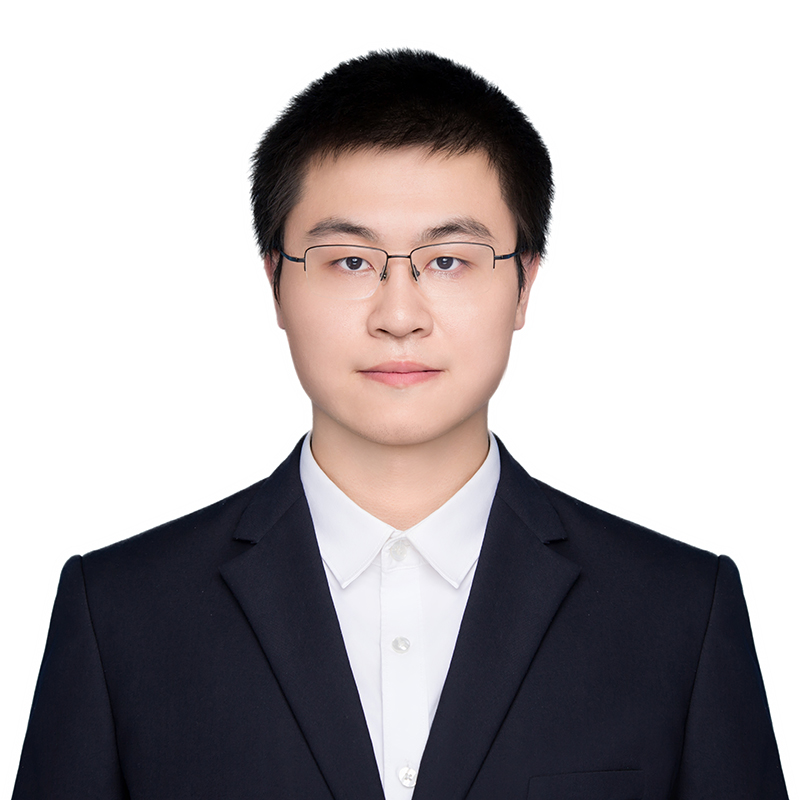
\includegraphics[width=0.88in]{photo.jpg}
\end{minipage}

\section{\faGraduationCap\  Education}
\datedsubsection{\textbf{Sun Yat-sen University}, Guangzhou}{2022 -- 2025}
\textit{M.Eng.} in Computer Vision\\
\href{https://www.sysu-hcp.net}{HCP Lab}, advised by Prof. Liang Lin \textit{(IEEE Fellow)}
\vspace{-0.3cm}
\datedsubsection{\textbf{Dalian University of Technology}, Dalian}{2018 -- 2022}
\textit{B.Eng.} in Electronic and Information Engineering\quad
GPA : 4.59/5, Rank \textcolor{red}{4}/206

\section{\faUsers\ Experience \& Research}

\datedsubsection{\textbf{LLM Evaluation (Tencent Hunyuan)}}{Jul 2025 -- Present}
\begin{itemize}
  \item \textbf{Benchmarks}: built \href{https://arxiv.org/abs/2605.26380}{\textbf{VisualNeedle}} (active visual search in information-dense scenes, whose counterfactual crop-black setting verifies a model really uses the evidence tools return), \href{https://hanxiao.io/jy-crpg-bench/}{\textbf{jy-crpg-bench}} (long-horizon play in an open-world RPG) and \href{https://arxiv.org/abs/2601.01400}{\textbf{EternalMath}} (a math benchmark that grows with human discovery)
  \item \textbf{Video scoring model}: split video quality into text--image consistency, visual quality and dynamic quality, built a 10k in-house dataset, and compared SFT, RL and frozen-scoring recipes on VLMs, reaching SOTA on in-house and public benchmarks (\href{https://arxiv.org/abs/2511.18825}{\textbf{Q-Save}})
\end{itemize}

\datedsubsection{\textbf{OpenRLHF: Alignment Algorithms \& Training Framework}}{Sep 2024 -- Present}
\begin{itemize}
  \item \textbf{Framework}: led the KL-loss algorithms in \href{https://github.com/OpenRLHF/OpenRLHF}{OpenRLHF} and built training backends including DeepSpeed AutoTP and FSDP2+CP+TP
  \item \textbf{Algorithm}: first identified that the \texttt{k3} estimator is biased when differentiated as a loss in GRPO, and proposed the unbiased \texttt{k2} loss; cited by \href{https://arxiv.org/abs/2501.03262}{Reinforce++} and expanded into \href{https://arxiv.org/abs/2510.01555}{\textbf{Rethinking KL Regularization in RLHF}}
\end{itemize}

\datedsubsection{\textbf{Diffusion-Based Adversarial Purification (HCP Lab, SYSU)}}{Mar 2023 -- Apr 2025}
\begin{itemize}
  \item \textbf{Analysis}: argued that diffusion purification defends through stochasticity rather than through forward noising shrinking the clean--adversarial KL divergence or a masking effect of Gaussian noise, and that its local loss landscape is not flat; first to separate this stochasticity from the one behind certified robustness
  \item \textbf{Method}: proposed diffusion denoising adversarial training, which smooths the loss landscape and improves robustness consistently across DDPM, DDIM, VP-SDE and EDM
\end{itemize}

\datedsubsection{\textbf{MMDetection Framework Development (Shanghai AI Lab)}}{Jul 2022 -- Mar 2023}
Core contributor to the Detection Transformer refactor across MMDetection 2.0 and 3.0
\begin{itemize}
  \item Simplified the registry and inheritance hierarchy and unified module data formats, improving readability, maintainability and runtime efficiency; MMDetection opened the branch \href{https://github.com/open-mmlab/mmdetection/tree/refactor-detr}{refactor-detr} for this work
  \item Re-implemented Conditional/DAB DETR and DINO, settled their naming and abstractions, aligned the reproduced metrics strictly and documented them; presented at an \href{https://www.bilibili.com/video/BV17x4y1w7ZK/?spm_id_from=333.337.search-card.all.click}{OpenMMLab community talk}
\end{itemize}

\section{\faPrint\ Publications}
{\small
\begin{itemize}
  \item \textbf{ICLR 2025}\quad \textit{(first author)} Towards Understanding the Robustness of Diffusion-Based Purification: A Stochastic Perspective
  \item \textbf{EMNLP 2025 Demo}\quad OpenRLHF: A Ray-based Easy-to-use, Scalable and High-performance RLHF Framework
  \item \textbf{ICASSP 2025}\quad Text Enhancement Network for Complex Multi-line Scene Text Image Super-resolution
  \item \textbf{Under review}\quad \textit{(second author)} jy-crpg-bench: A Long-Horizon Benchmark for Frontier Models in an Open-World RPG
  \item \textbf{Under review}\quad \textit{(co-first author)} VisualNeedle: Benchmarking Active Visual Search in Information-Dense Scenes
  \item \textbf{arXiv}\quad Rethinking KL Regularization in RLHF: From Value Estimation to Gradient Optimization
  \item \textbf{arXiv}\quad Q-Save: Towards Scoring and Attribution for Generated Video Evaluation
  \item \textbf{arXiv}\quad EternalMath: A Living Benchmark of Frontier Mathematics that Evolves with Human Discovery
  \item \textbf{arXiv}\quad DramaChain Bench: An End-to-End Benchmark for Short-Drama Generation
\end{itemize}
\par}

\section{\faCogs\ Skills}
\begin{itemize}
  \item Interests: LLM evaluation (benchmark design, automatic scoring and attribution), Agentic RL
  \item Training: DTensor-based FSDP2 parallelism, DeepSpeed, Ray + vLLM RLHF stack
\end{itemize}

\end{document}
